\chapter{Aplikacje klienckie}

\section*{Aplikacja Android}

Opis Androida, screenshoty


\section*{Aplikacja iOS}

Opis iOS, screenshoty

Aplikacja przeznaczona jest na urządzenia z systemem operacyjnym iOS od wersji 10.0. 
Nie wspiera ona wcześniejszych wersji ze względu na nowe funkcje, które Apple wprowadziło wraz z pojawieniem się iOS 10.0 (m.in. klasa UNUserNotificationCenter). Jednak jak wynika z wykresu niżej (numer rysunku) 92\% wszystkich obecnych użytkowników tego systemu jest w stanie zainstalować aplikację a liczba ta stale rośnie. Aplikacja wykonana została wspierając zarówno telefony komórkowe iPhone jak i tablety iPad. 
\begin{figure}[h]
	\centering
	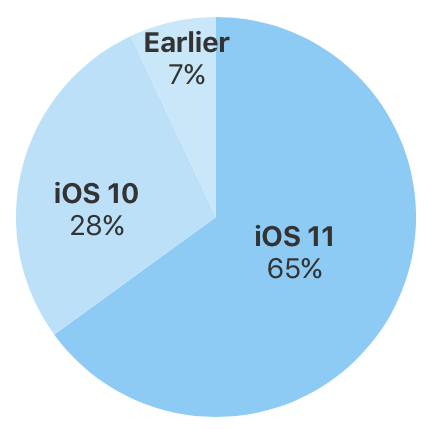
\includegraphics[width=6cm]{iOSstat}
	\caption{Udziały wersji systemu iOS w rynku}
\end{figure}

Architektura:
Aplikacja napisana jest w stosunkowo nowym języku Swift(został zaprezentowany przez Apple w 2014r na konferencji WWDC) w oparciu o architekturę MVC (Model-View-Controller) wykorzystując przy programowanie reaktywne i funkcjonalne. 
Instalacja zewnętrzynych bibliotek odbywa się za pomocą CocoaPods. Jest to menadżer zależności dzięki któremu szybko możemy wyszukać i zainstalować wymagane oprogramowanie.




\section*{Aplikacja internetowa}

Opis weba, screenshoty